\section{Algorithms for Gradient-Based Optimization}

Gradient-based optimization underpins the training of neural networks. The objective is to identify a parameter set $\theta \in \mathbb{R}^d$ that minimizes a scalar loss function $J(\theta)$. Given that an analytical solution for $\nabla J(\theta) = 0$ is intractable for high-dimensional non-convex surfaces, iterative numerical methods are required.

\subsection{Gradient Descent}

Standard Gradient Descent (GD) iteratively updates parameters in the direction of the negative gradient, $-\nabla J(\theta)$, representing the steepest descent. The update rule for iteration $t$ with learning rate $\eta$ is:
\begin{equation}
    \theta_{t+1} = \theta_t - \eta \nabla J(\theta_t)
\end{equation}

\begin{figure}[h]
	\centering
	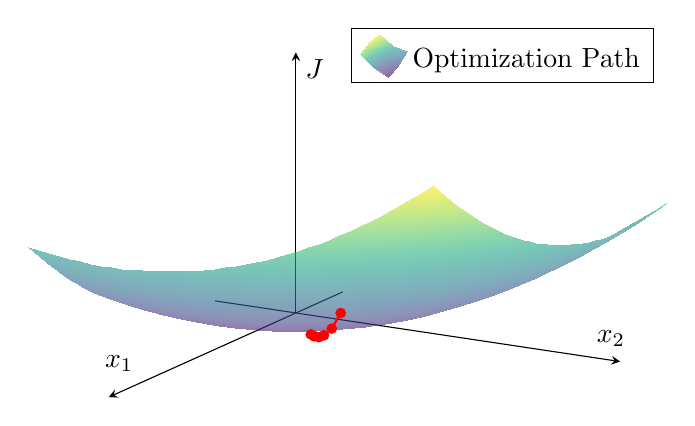
\begin{tikzpicture}
		\begin{axis}[
			width=0.8\textwidth, % Slightly responsive width
			height=7cm,
			axis lines=middle,
			xlabel={$x_1$}, ylabel={$x_2$}, zlabel={$J$},
			xtick=\empty, ytick=\empty, ztick=\empty, % Cleaner look
			grid=major, grid style={dashed, gray!30},
			view={120}{25}, % Better viewing angle
			colormap/viridis,
			]
			
			% Cost function surface
			\addplot3[domain=-1:4, domain y=-1:4, samples=40, surf, opacity=0.6, shader=interp] 
                {0.5*(x^2 + y^2)};
			
			% Trajectory
			\addplot3[thick, red, mark=*, mark size=1.5pt] coordinates {
				(3.2,2.4,5.92) (2.56,1.92,3.78) (2.05,1.53,2.42)
				(1.64,1.23,1.55) (1.31,0.98,0.99) (1.05,0.79,0.63)
			};
			\addlegendentry{Optimization Path}
		\end{axis}
	\end{tikzpicture}
	\caption{Visualization of the Gradient Descent trajectory on a convex error surface.}
	\label{fig:gradient_descent}
\end{figure}

\subsection{Optimization Variants}

Standard GD computes the gradient over the full dataset $\mathcal{D}$, which is computationally prohibitive for large-scale learning. Modern variants address computational efficiency and convergence speed.

\setlength{\columnsep}{1cm}
\begin{multicols}{2}

\subsubsection{Stochastic Gradient Descent (SGD)}
SGD approximates the full gradient using a \textit{mini-batch} $\mathcal{B} \subset \mathcal{D}$ of size $m$. The approximate loss is:
\begin{equation}
    J_{\mathcal{B}}(\theta) = \frac{1}{m} \sum_{(x,y) \in \mathcal{B}} L(f(x;\theta), y)
\end{equation}
While $\mathbb{E}[\nabla J_{\mathcal{B}}(\theta)] = \nabla J(\theta)$, the introduced variance (noise) acts as a regularizer, aiding the escape from local minima (saddle points).

\subsubsection{Momentum}
To mitigate oscillation in high-curvature areas, Momentum accumulates a velocity vector $v_t$, effectively averaging past gradients \citep{Rumelhart1986}:
\begin{align}
    v_{t+1} &= \mu v_t - \eta \nabla J(\theta_t) \\
    \theta_{t+1} &= \theta_t + v_{t+1}
\end{align}
where $\mu \in [0, 1)$ is the momentum coefficient.

\subsubsection{Nesterov Accelerated Gradient}
Nesterov (NAG) improves momentum by computing the gradient at the \textit{anticipated} future position:
\begin{equation}
    v_{t+1} = \mu v_t - \eta \nabla J(\theta_t + \mu v_t)
\end{equation}
This "look-ahead" capability provides a correction factor that improves convergence rates near the optimum.

\subsubsection{Adam}
Adaptive Moment Estimation (Adam) adapts the learning rate per parameter. It estimates the first ($m_t$) and second ($v_t$) raw moments of the gradients:
\begin{align}
    m_t &= \beta_1 m_{t-1} + (1 - \beta_1) g_t \\
    v_t &= \beta_2 v_{t-1} + (1 - \beta_2) g_t^2
\end{align}
where $g_t = \nabla J(\theta_t)$. Bias-corrected estimates $\hat{m}_t$ and $\hat{v}_t$ are used for the update:
\begin{equation}
    \theta_{t+1} = \theta_t - \eta \frac{\hat{m}_t}{\sqrt{\hat{v}_t} + \epsilon}
\end{equation}
Adam is currently the standard for deep learning due to its robustness to sparse gradients and stationary objectives.

\end{multicols}